\section{Ciclo de vida de un producto}
\begin{itemize}
    \item Una marca tiene personalidad, un producto tiene una personalidad también.
    \item Así como una persona el producto nace, se reproduce y muere.
\end{itemize}

%----------------------------------------------------------------------------------------
\subsection{Ejemplos}
\begin{itemize}
    \item Zurich y Sears en declive.
\end{itemize}


%%%%%%%%%%%%%%%%%%%%%%%%%%%%%%%%%%%%%%%%%%%%%%%%%%%%%%%%%%%%%%%%%%%%%%%%%%%%%%%%%%%%%%%%%%
\section{Etapas del ciclo de vida de un producto}
\textbf{Consideraciones preliminares:}
\begin{itemize}
    \item La etapa preliminar a esta gráfica es enorme.
\end{itemize}

\textbf{Etapas:}
\begin{figure}[htbp]
    \centering
    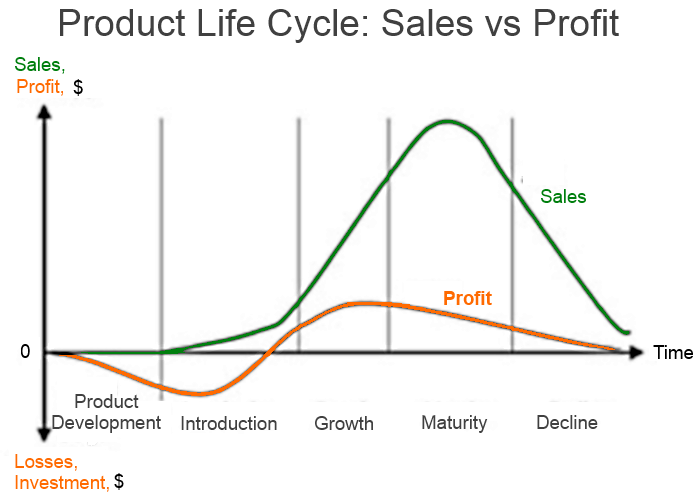
\includegraphics[width=12cm]{./../__Imagenes__/2020-02-27_00.png}
    \caption{Curva de ciclo de vida de un producto}
    \label{}
\end{figure}
\begin{enumerate}
    \item Product development: 
        \begin{itemize}
            \item Los ingresos suben, pero por el gasto hay un ligero declive en las ganancias. 
            \item Definir estrategia, trueques, target.
            \item Crear un modelo de negocio.
        \end{itemize}
        
    \item Introduction: 
        \begin{itemize}
            \item Conciencia de tu existencia en el mercado a los consumidores.
            \item Generar pruebas, oséa prototipar, introducir Producto Mínimo Viable (PMV ó MVP).
            \item Crecer con demanda.
        \end{itemize}

    \item Growth: 
        \begin{itemize}
            \item Construir la marca, trabajar en posicionamiento.
            \item Maximizar share.
            \item Ampliar surtido.
        \end{itemize}

    \item Maturity: 
        \begin{itemize}
            \item Proteger el market share, intentar ganar a la competencia.
            \item Buscar eficiencia operativa.
            \item Eliminar debilidades.
            \item Extensiones de marca hacia otras categorías, extensión.
        \end{itemize}

    \item Decline: 
        \begin{itemize}
            \item Buscar nuevos usos por el producto. 
            \item Buscar nuevos mercados.
            \item Innovar / investigar, de esto depende la pendiente negativa de este declive.
        \end{itemize}
\end{enumerate}
